
性能是设计目标之一,与其他需求同等重要。因此,“这种设计导致了糟糕的性能”问题的回答与“这种设计没有提供我们需要的功能”问题的答案是一样的。两种情况下,都需要不同的设计。只是更习惯于根据他们做的怎么样来评估设计,而不是做得有多快。

为了在第一次尝试时,选择性能提升设计实践,现在介绍几个专门针对良好性能的设计指南。它们也是可靠的设计原则,有理由去了解它们,遵循这些原则不会让设计变得更糟。 

前两条指导原则处理设计中不同组件(函数、类、模块、过程、任何组件)的交互。首先,建议交互传递尽可能少的信息,以便整个系统能正常工作。其次,建议不同的组件提供尽可能多的关于交互预期结果的信息。如果认为这是一组矛盾,也没什么问题。设计通常是解决矛盾的艺术,两个矛盾的陈述都正确,只是时间或空间不同。下面的例子很好地说明了这种(更普遍的)管理设计矛盾的方法。

\subsubsubsection{12.3.1\hspace{0.2cm}最小信息原则}

从第一条准则开始。尽可能少地交互信息,上下文在这里非常重要,建议组件尽可能少地暴露它如何处理特定请求的信息。组件之间的交互是由约定控制的。当讨论类和函数的接口时,已经习惯了这个想法,但它是一个更广泛的概念,用比如于两个进程之间通信的协议,这就是一个约定。 

在此类接口或交互中,作出和履行承诺的一方不应提供额外的信息。看一些具体的例子,将从实现基本队列的类开始,然后问自己。从效率的角度来看,什么是好的接口?

其中有一个方法允许检查队列是否为空。注意,调用者并没有询问队列有多少元素,而只是询问队列是否为空。虽然队列的某些实现可能会缓存大小,并将其与0进行比较以应对此请求。但对于其他实现,确定队列是否为空可能比计算元素更有效。约定中,“如果队列为空,将返回true。”即使知道大小,也不要做承诺:\textit{不要主动提供额外的信息}。这样,后面就可以自由地更改实现了。 

类似地,入队和出队的方法应该只保证向队列中添加或删除新元素。从队列中弹出一个元素,必须处理空队列的情况,或者声明未定义尝试的结果(STL选择的方法)。可能注意到,STL队列从效率的角度展示了一个出色的接口,其完成了对队列数据结构的约定,而没有透露任何不必要的细节。特别是,\texttt{std::queue}是一种适配器,可以在几个容器中的一个上实现。队列可以实现为\texttt{vector}、\texttt{deque}或\texttt{list},这个例子告诉我们,接口需要隐藏实现细节。

对于接口泄漏太多实现信息的反面例子,考虑另一个STL容器,无序\texttt{set}(或\texttt{map})。\texttt{std::unor\break dered\_set}容器有一个接口,允许插入新元素并检查给定的值是否已经在集合中(目前为止,一切正常)。根据定义,它缺乏元素的内部顺序,并且标准提供的性能保证清楚地表明数据结构使用了哈希。所以,接口中显式地引用哈希的部分是必要的,所以必须指定一个用户给定的哈希函数。但是这个接口走远了,通过像\texttt{bucket\_count()}这样的方法,暴露了底层实现必须是一个带有桶的离散链接哈希表,以解决哈希冲突。因此,不可能使用开放寻址哈希表创建一个完全符合STL的无序\texttt{set}。此接口限制了实现,并可能阻碍使用更高效的实现。

虽然在简单的例子中使用了类设计,但同样的原则也可以应用于更大模块的API,客户端-服务器协议,以及系统组件之间的其他交互。在设计响应请求或提供服务的组件时,只需提供简洁的约定,并只显示请求者所需的信息即可。

最小信息或最小承诺的设计准则,本质上是对类接口设计准则的概括:\textit{接口不应暴露实现}。此外,要考虑到纠正违反这条指导原则的行为会相当困难。若设计泄露了实现细节,那么客户将依赖于它们,并且若更改了实现,就会破坏客户的代码。因此,为性能而设计与一般的设计实践一样。在下一个指导方针中,我们将开始介绍不同设计目标和相应最佳实践之间的关系。

\subsubsubsection{12.3.2\hspace{0.2cm}最大信息原则}

虽然完成请求的组件应该避免暴露可能限制实现的信息,但对于发出请求的组件来说,情况正好相反。请求者或调用者应该能够提供关于具体需要什么的特定信息。当然,调用方只有在有合适的接口时才提供信息,因此接口应该允许这样的“完整”请求。

特别是,要提供最佳性能,了解请求背后的意图通常很重要。同样,通过一个例子,应该会更容易理解这个概念。
 
让我们从一个随机访问序列容器开始。随机访问可以访问容器中的任意第\texttt{i}个元素,而不需要访问其他元素。通常的方法是使用索引运算符:

\begin{lstlisting}[style=styleCXX]
T& operator[](size_t i) { return … i-th element …; }
\end{lstlisting}

有了这个操作符,就可以遍历容器了:

\begin{lstlisting}[style=styleCXX]
container<T> cont;
… add some data to cont …
for (size_t i = 0; i != cont.size(); ++i) {
	T& element_i = cont[i];
	… do some work on the i-th element …
}
\end{lstlisting}

从效率的角度来看,这不是最好的方法,因为现在使用随机访问迭代器进行顺序迭代。对于更强大或功能更强大的接口,在只使用了它的一小部分功能时,就应该关注效率。该接口的灵活性可能会以性能为代价,如果不使用这些特性,就会浪费性能。 

假设\texttt{std::deque}是一个支持随机访问的块分配容器。为了访问任意元素\texttt{i},必须首先计算哪个块包含这个元素(通常是一个取模操作)和块中元素的索引,然后在辅助数据结构(块指针表)中找到块的地址,并在块中进行索引。对于下一个元素,必须重复这个过程。不过在大多数情况下,元素将驻留在同一个块中,而且我们对地址已知。这是因为对任意元素的请求没有包含足够的信息,没有办法知道将很快请求下一个元素。因此,\texttt{deque}不能以最有效的方式处理遍历。

另一种遍历整个容器的方法是使用迭代器:

\begin{lstlisting}[style=styleCXX]
for (auto it = cont.begin(); it != cont.end(); ++it) {
	T& element = *it;
	… do some work on the element …
}
\end{lstlisting}

\texttt{deque}的实现者可以假设迭代器的自增(或自减)操作。因此,如果有一个迭代器\texttt{it}并访问相应的元素\texttt{*it},很可能会请求下一个元素。\texttt{deque}迭代器可以在块指针表中存储块指针或右变元素的索引,这将使访问一个块中元素的成本更低。通过一个简单的基准测试,可以验证使用迭代器遍历\texttt{deque}容器确实比索引更快:

\hspace*{\fill} \\ %插入空行
\noindent
\textbf{01\_deque.C}
\begin{lstlisting}[style=styleCXX]
void BM_index(benchmark::State& state) {
	const unsigned int N = state.range(0);
	std::deque<unsigned long> d(N);
	for (auto _ : state) {
		for (size_t i = 0; i < N; ++i) {
			benchmark::DoNotOptimize(d[i]);
		}
		benchmark::ClobberMemory();
	}
	state.SetItemsProcessed(N*state.iterations());
}
void BM_iter(benchmark::State& state) {
	const unsigned int N = state.range(0);
	std::deque<unsigned long> d(N);
	for (auto _ : state) {
		for (auto it = d.cbegin(), it0 = d.cend(); 
		it != it0; ++it) {
			benchmark::DoNotOptimize(*it);
		}
		benchmark::ClobberMemory();
	}
	state.SetItemsProcessed(N*state.iterations());
}
\end{lstlisting}

性能差异显著:

\hspace*{\fill} \\ %插入空行
\begin{center}
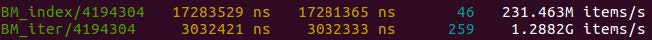
\includegraphics[width=0.9\textwidth]{content/3/chapter12/images/1.jpg}\\
图12.1 - 使用索引和迭代器遍历\texttt{std::deque}
\end{center}

指出为性能而设计和为性能而优化之间的关键区别非常重要。不能保证迭代器访问\texttt{deque}容器的速度更快,特定的实现可能会使用索引操作符来实现迭代器,这样的保证可能来自一个优化的实现。本章中,我们感兴趣的是设计。尽管,谈论“有效的设计”时,其他人可能会理解这话的意思,但设计不能真正地“优化”。设计可以允许或阻止某些优化,所以更准确的说法是“性能敌对”或“性能友好”的设计(后者通常也称为有效设计)。

在\texttt{deque}示例中,索引操作符对于随机访问是高效的,并且将顺序迭代视为随机访问的一种特殊情况。调用者不可能说:“接下来我可能会请求相邻的元素。”相反,根据迭代器的存在性,可以推断它可能是递增或递减的。该实现可以使这种增量操作执行的更高效。

进一步讨论容器的例子。这一次,考虑一个自定义容器,功能上是一个树,但与\texttt{std::set}不同,不将值存储在树节点中。相反,将值存储在序列容器(数据存储)中,而树节点包含指向该容器元素的指针。树本质上是数据存储的索引,因此需要一个定制的比较函数。这里想要比较的是值,而不是指针。

\hspace*{\fill} \\ %插入空行
\noindent
\textbf{02\_index\_tree.C}
\begin{lstlisting}[style=styleCXX]
template<typename T> struct compare_ptr {
	bool operator()(const T* a, const T* b) const {
		return *a < *b;
	}
};
template <typename T> class index_tree {
	public:
	void insert(const T& t) { 
		data_.push_back(t);
		idx_.insert(&(data_[data_.size() - 1]));
	}
	private:
	std::set<T*, compare_ptr<T>> idx_;
	std::vector<T> data_;
};
\end{lstlisting}

插入新元素时,将添加到数据存储的末尾,而指针将添加到由元素比较确定的索引位置。为什么要选择这样的实现,而不是\texttt{std::set}呢?某些情况下,可能会有强制的需求,例如:数据存储可能是磁盘上的内存映射文件。其他情况下,为了提高性能,可以选择这种实现。可能乍一看,额外的内存使用和通过指针间接访问元素会降低性能。 

为了了解这个索引树容器的性能优势,检查搜索满足给定谓词的元素的操作。假设容器提供了迭代器,可以简单地遍历索引集,就可以轻松地进行搜索。解引用操作符应该返回索引的元素值,而不是指针:

\hspace*{\fill} \\ %插入空行
\noindent
\textbf{02\_index\_tree.C}
\begin{lstlisting}[style=styleCXX]
template <typename T> class index_tree {
	using idx_t = typename std::set<T*, compare_ptr<T>>;
	using idx_iter_t = typename idx_t::const_iterator;
	public:
	class const_iterator {
		idx_iter_t it_;
		public:
		const_iterator(idx_iter_t it) : it_(it) {}
		const_iterator operator++() { ++it_; return *this; }
		const T& operator*() const { return *(*it_); }
		friend bool operator!=(const const_iterator& a,
		const const_iterator& b) {
			return a.it_ != b.it_;
		}
	};
	const_iterator cbegin() const { return idx_.cbegin(); }
	const_iterator cend() const { return idx_.cend(); }
	…
};
\end{lstlisting}

要确定一个满足特定要求的值是否已经存储在容器中,只需遍历整个容器,并检查每个值的谓词:

\begin{lstlisting}[style=styleCXX]
template <typename C, typename F> bool find(const C& c, F f) {
	for (auto it = c.cbegin(), i0 = c.cend(); it != i0; ++it) {
		if (f(*it)) return true;
	}
	return false;
}
\end{lstlisting}

当使用迭代器访问容器时,我们向容器提供了什么信息?告诉它我们打算每次访问下一个元素。我们并没有告诉它这样做的原因,并且原因重要吗?在这种情况下,确实如此。仔细想象需要做什么,需要访问容器中的每个元素,直到找到满足给定条件的元素。如果这看起来像是在重述同样的事情,那你还没教条化。这个需求中,没有说要按顺序访问容器元素,只是说需要遍历所有元素。如果有一个API,它告诉容器检查所有元素,但不要求特定的顺序,容器就可以自由地优化访问顺序。对于索引容器,最优的访问顺序是遍历数据存储本身,这就提供了最佳的内存访问模式(顺序访问)。在我们的例子中,元素在存储中的实际顺序,就是它们添加的顺序,但这无关紧要。我们要求返回的只是一个布尔值,甚至不询问匹配元素的位置。换句话说,虽然可能有多个元素满足这个条件,但调用者想知道是否存在一个这样的元素。我们没有请求元素或任何特定元素的值,这是“查找任意一个”的请求,而不是“先查找”的请求。 

下面的版本用的是这种接口,允许调用者提供所有相关信息和可能的实现:

\hspace*{\fill} \\ %插入空行
\noindent
\textbf{02\_index\_tree.C}
\begin{lstlisting}[style=styleCXX]
template <typename T> class index_tree {
	…
	template <typename F> bool find(F f) const {
		for (const T& x : data_) {
			if (f(x)) return true;
		}
		return false;
	}
};
\end{lstlisting}

快吗?基准测试可以回答这个问题。如果该值未找到,或很少找到,则这种性能差异会更为明显:

%\hspace*{\fill} \\ %插入空行
\begin{center}
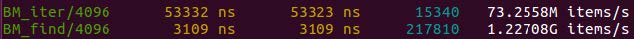
\includegraphics[width=0.9\textwidth]{content/3/chapter12/images/2.jpg}\\
图12.2 - 使用迭代器和\texttt{find()}成员函数在索引数据存储中进行搜索
\end{center}

退一步评估这个例子是非常重要的,它是软件设计的经验,而不是一个特定的优化技术。这个上下文中,\texttt{find()}成员函数是否比基于迭代器的搜索快得多并不重要。在设计阶段,重要的是适当的实现可能会更快。它可能更快的原因是因为知道调用者的意图。 

使用非成员和成员\texttt{find()}比较调用者提供的信息,当非成员\texttt{find()}函数调用容器接口时,我们告诉容器:“依次查看所有容器元素的值。”实际上并不需要这些操作,但这是给容器的信息,因为这是能通过迭代器接口传递的唯一信息。另一方面,成员\texttt{find()}允许发出以下请求:“以任意顺序检查所有元素,并告诉我是否至少有一个元素符合这个条件。”这个请求施加的限制要少得多,其将细节留给容器本身。在我们的示例中,实现者利用这种自由提供了更好的性能。

设计阶段,可能不知道这样的优化实现。成员\texttt{find()}的第一个实现也可以运行迭代器循环或调用\texttt{std::find\_if}。开发者也可能永远不会优化这个函数,因为在应用程序中很少调用,并且不是性能瓶颈。但是软件系统的寿命往往比预期的要长,而且重新设计是困难和耗时的。好的系统架构不应该限制系统的发展,甚至可以满足添加新的特性和性能需求。

再次看到了性能友好型和性能敌对型设计之间的区别。当然,同样的原则也适用于系统组件之间的交互,而不限于类。在设计响应请求或提供服务的组件时,允许请求者提供所有相关的信息,特别是表达请求背后的意图。

由于几个原因,这是一个更有争议性的指南。首先,明显地违背了类设计的主流方法:永远不要为不需要特权访问,且完全可以通过现有的公共API实现的任务实现(public)成员函数。关于这个问题,了解一下这样做的几个理由。首先,有人可能会说“可以以十倍的速度实现”并不真正符合“可以实现”的标准,因此该指导方针并不适用。相反,在设计阶段甚至可能不知道需要这种性能。我们可能会违反的另一个重要规则是“不要过早地优化”,尽管不应该简单地理解这条规则,这条规则的合理支持者经常会补充说,“但也不要过早地悲观”。后者在设计的背景下,意味着做出设计决策,封闭未来的优化空间。

最大信息原则(或信息丰富的接口)的使用是一个平衡和合理判断的问题。考虑到这一点,违反这条原则远不如不遵守前面的规则那么有害。若接口或约定暴露了不必要的信息,那么很难从依赖它的客户端收回这些信息。另一方面,如果接口不允许客户端提供相关的意图信息,那么客户端可能会执行低效率的实现。但在添加了信息更丰富的接口之后,一切就不同了,客户端可以根据需要转换到这个接口上。

因此,决定是否在一开始就提供一个信息丰富的接口,取决于以下几个因素: 

\begin{itemize}
\item 
这个组件或组件之间的交互对性能至关重要的可能性有多大?虽然不鼓励猜测特定代码的性能,但需要知道有关组件的一般需求。每秒访问数百万次的数据库很可能成为某个地方的性能瓶颈,而每月为员工提供两次发薪地址的系统可以进行保守地设计,并在需要时再进行优化。

\item 
这个设计决策的影响有多大?若低效的实现泛滥,那当添加一个新的、更高级别的接口时,替换的难度有多大?一个类使用一到两次,可以很容易地随着它的客户端更新。一个通信协议将成为整个系统的标准,并用于一个轻量级协议API中,该API将消息存储在磁盘上长达数周或数月,从一开始就应该具有可扩展性,包括用于未来更丰富信息请求的选项。
\end{itemize}

通常情况下,这些选择并不明确,取决于设计师的直觉和经验。本书对前者有帮助,在实践中可以解决后者的问题。 

在考虑不同设计决策的性能影响时,我们经常关注接口和数据组织。在下面的两个部分中,我们将展开讨论这两个主题,从接口设计开始。








